\chapter{Analysis and comments}
\indent
	Different optimizers, activation functions, learning rates, and dimension of hidden layers are tested in this chapter. 
	Experiments of this chapter are done with common setup below: 
	\begin{itemize}
		\item Seed: 42.
		\item Number of hidden layers: 2.
	\end{itemize} 

\section{Different optimizers}
\indent
	Experiments of this section are done with common setup below: 
	\begin{itemize}
		\item Activation function: \code{LeakyReLU}.
		\item Learning rate: $10^{-2}$.
		\item Dimension of hidden layers: 4.
	\end{itemize}

	From Figures \ref{result-optim-adam} and \ref{result-optim-vanilla}, we can see that 
	using \code{Adam} optimizer makes the model converge faster in this case.
	
	\begin{figure}[H]
		\centering
		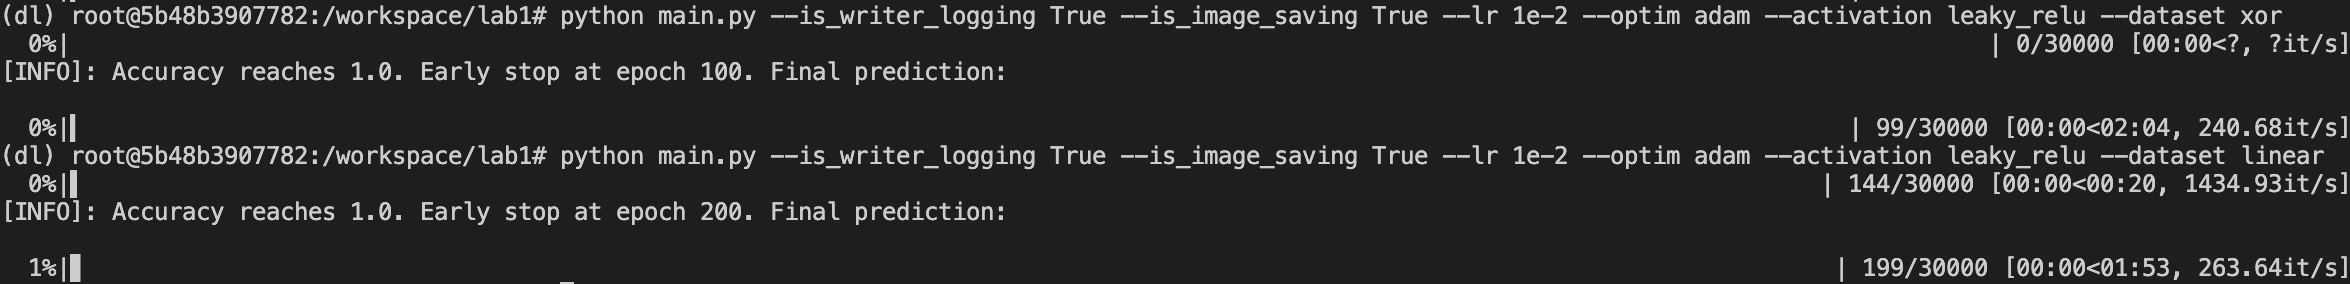
\includegraphics[scale=0.35]{img/adam_1e-2_leaky-relu.png}
		\caption{Results with Adam optimizer. In this case, the model converges in less than 100 and 200 epochs, respectively.}
		\label{result-optim-adam}
	\end{figure}
	\begin{figure}[H]
		\centering
		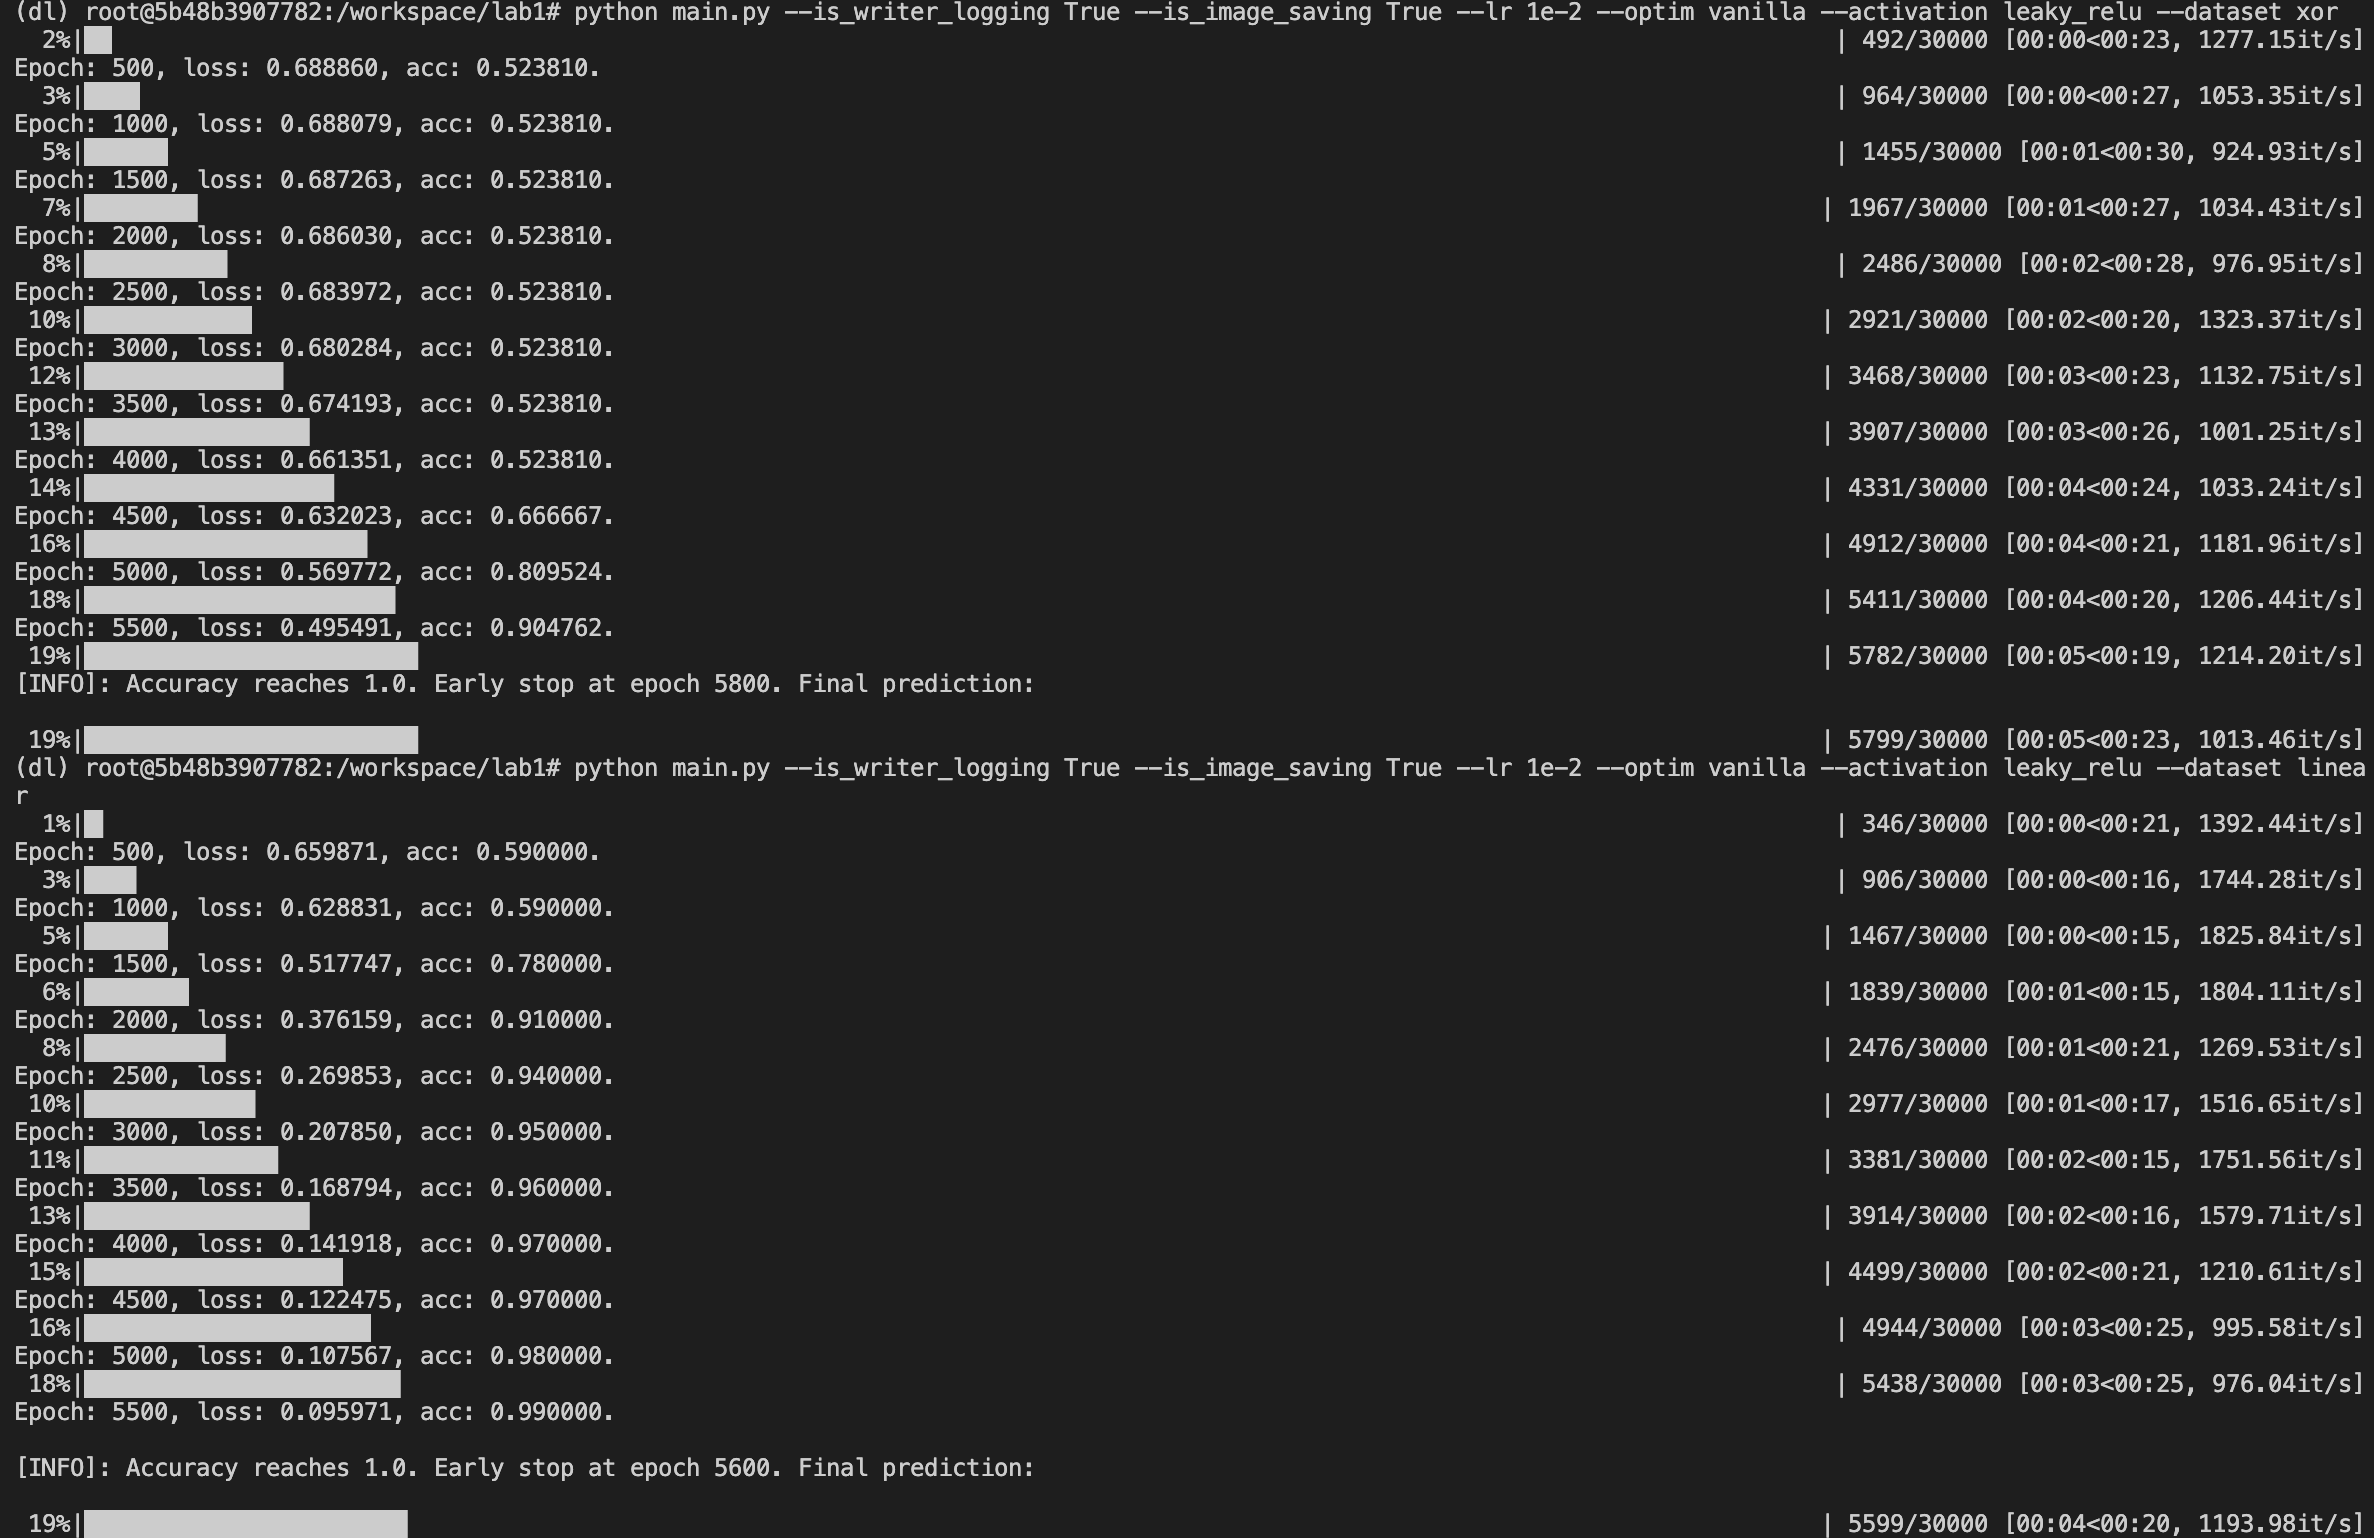
\includegraphics[scale=0.35]{img/vanilla_1e-2_leaky-relu.png}
		\caption{Results with SGD optimizer. In this case, the model converges in less than 5800 and 5600 epochs, respectively.}
		\label{result-optim-vanilla}
	\end{figure}

	\begin{figure}[H]
		\centering
		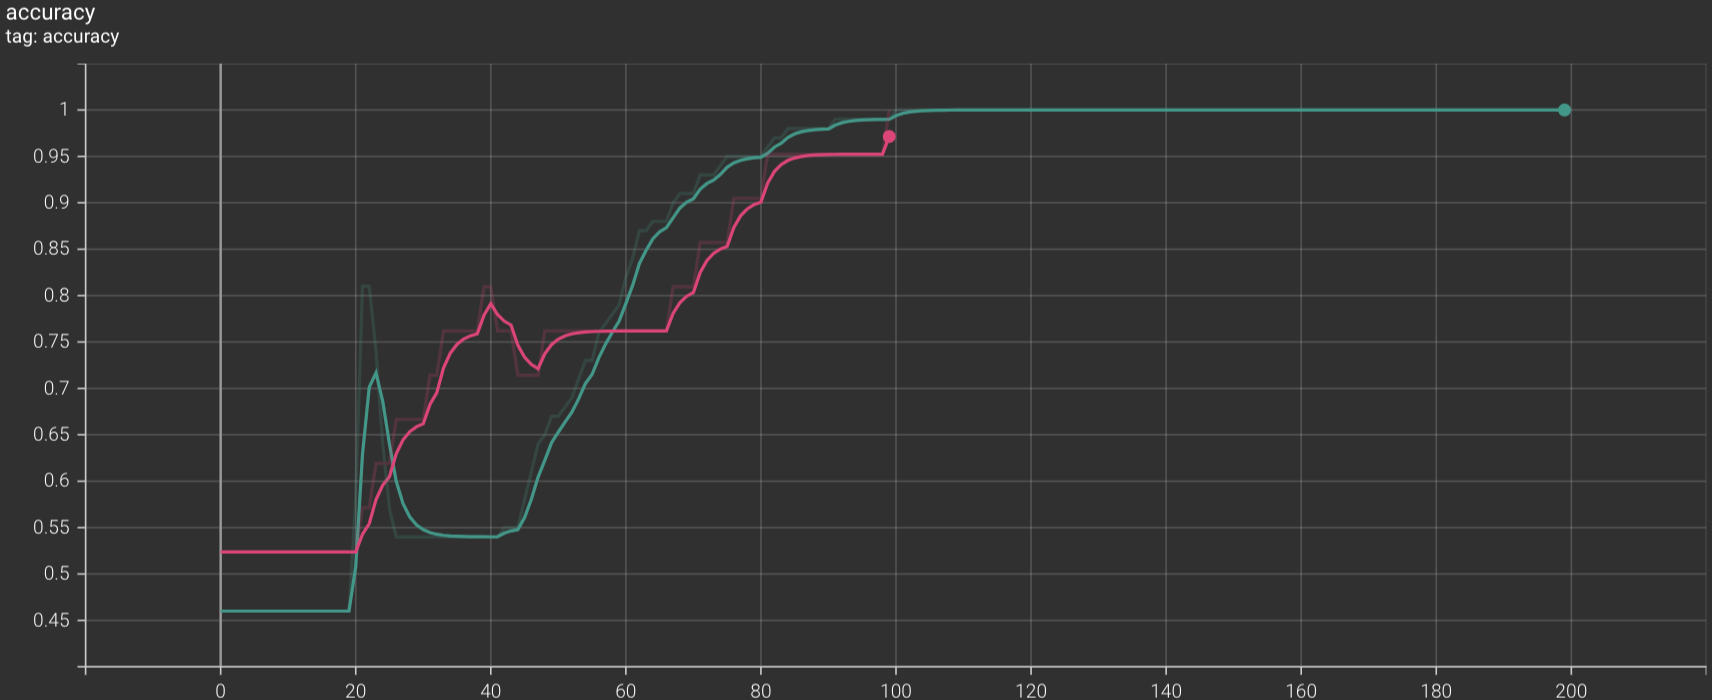
\includegraphics[scale=0.5]{img/adam_acc.png}
		\caption{Accuracy with Adam optimizer.}
		\label{optim-acc-adam}
	\end{figure}
	\begin{figure}[H]
		\centering
		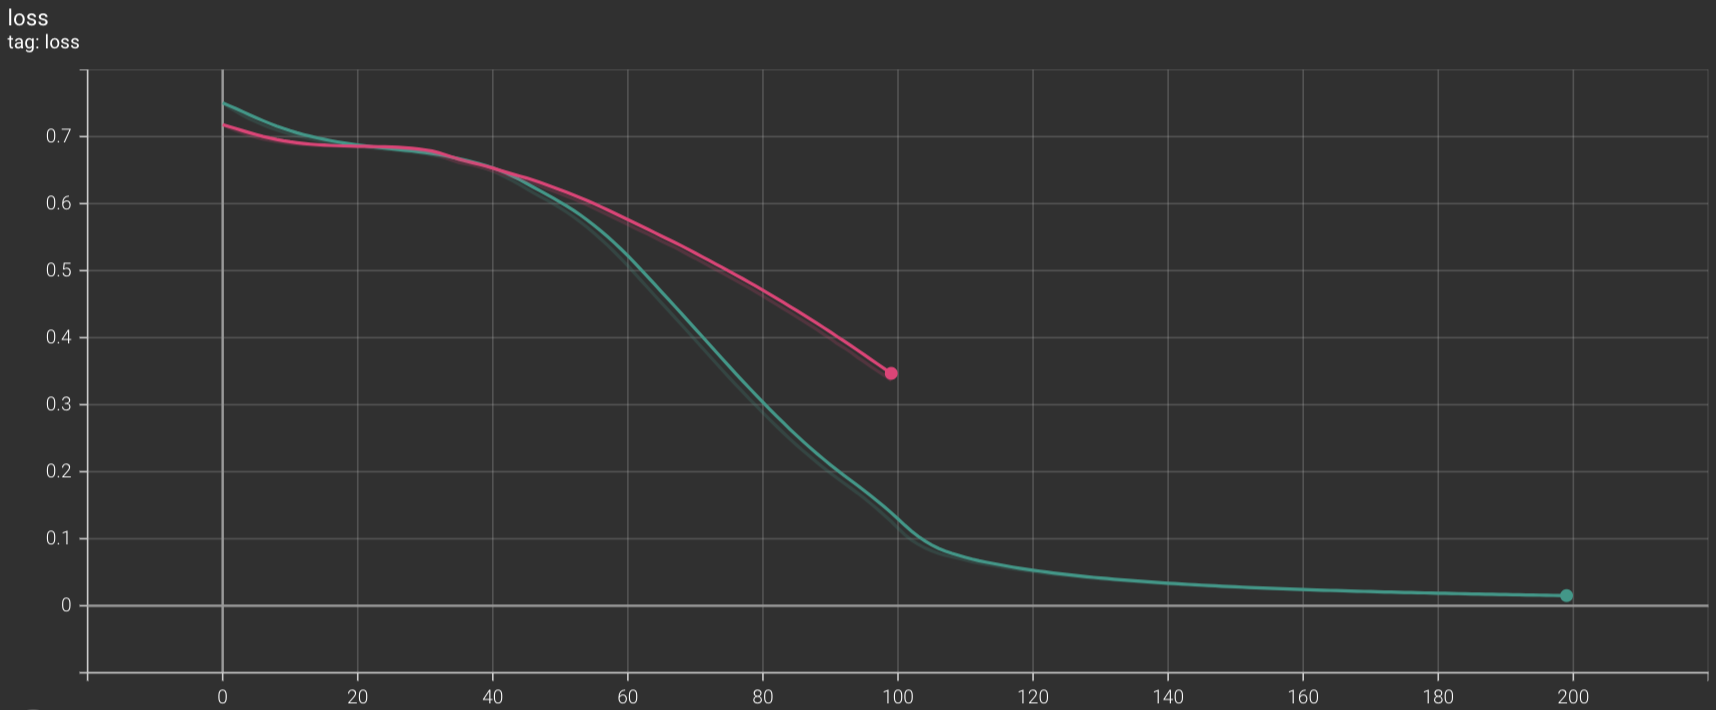
\includegraphics[scale=0.5]{img/adam_loss.png}
		\caption{Loss with Adam optimizer.}
		\label{optim-loss-adam}
	\end{figure}

	\begin{figure}[H]
		\centering
		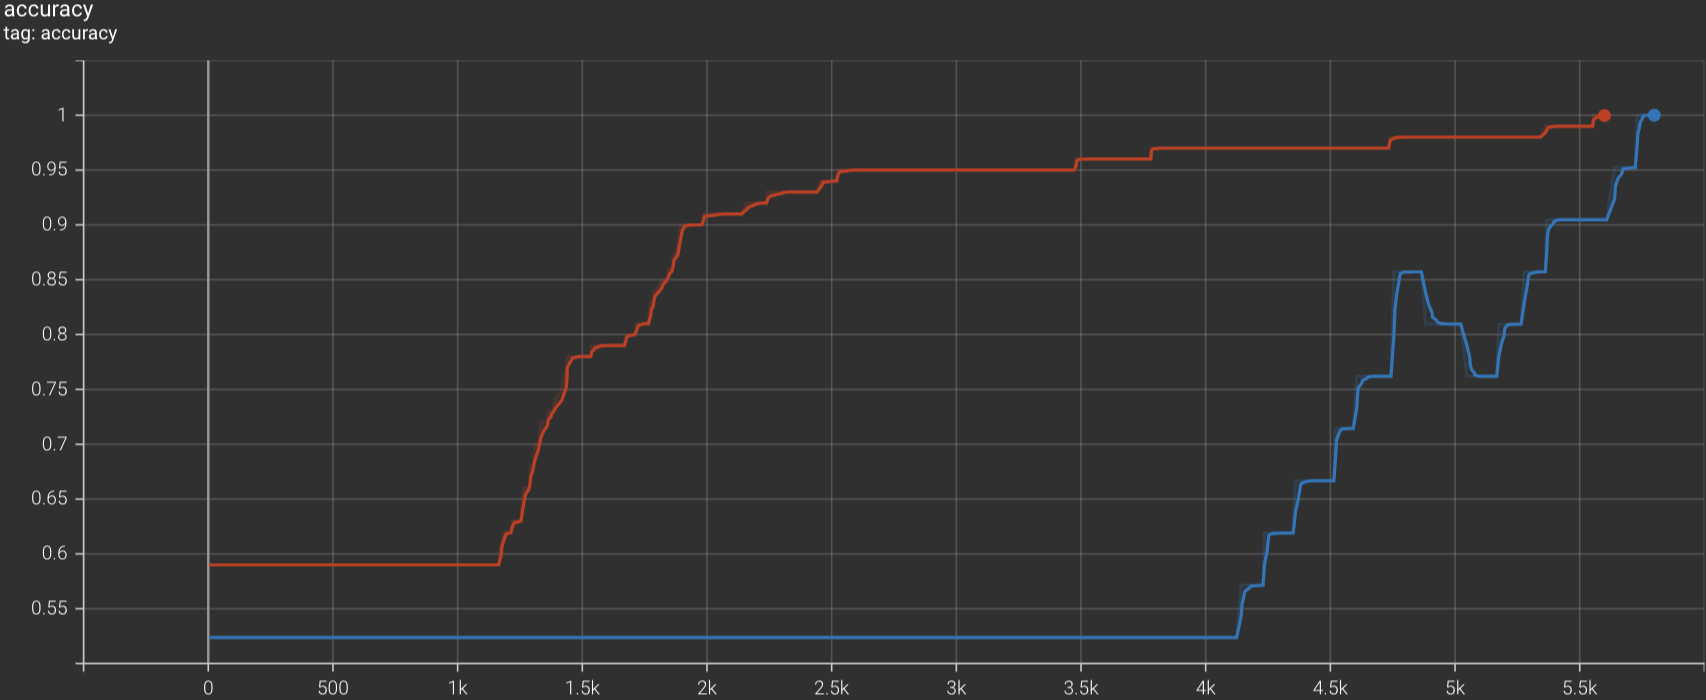
\includegraphics[scale=0.5]{img/vanilla_acc.png}
		\caption{Accuracy with SGD optimizer.}
		\label{optim-acc-vanilla}
	\end{figure}
	\begin{figure}[H]
		\centering
		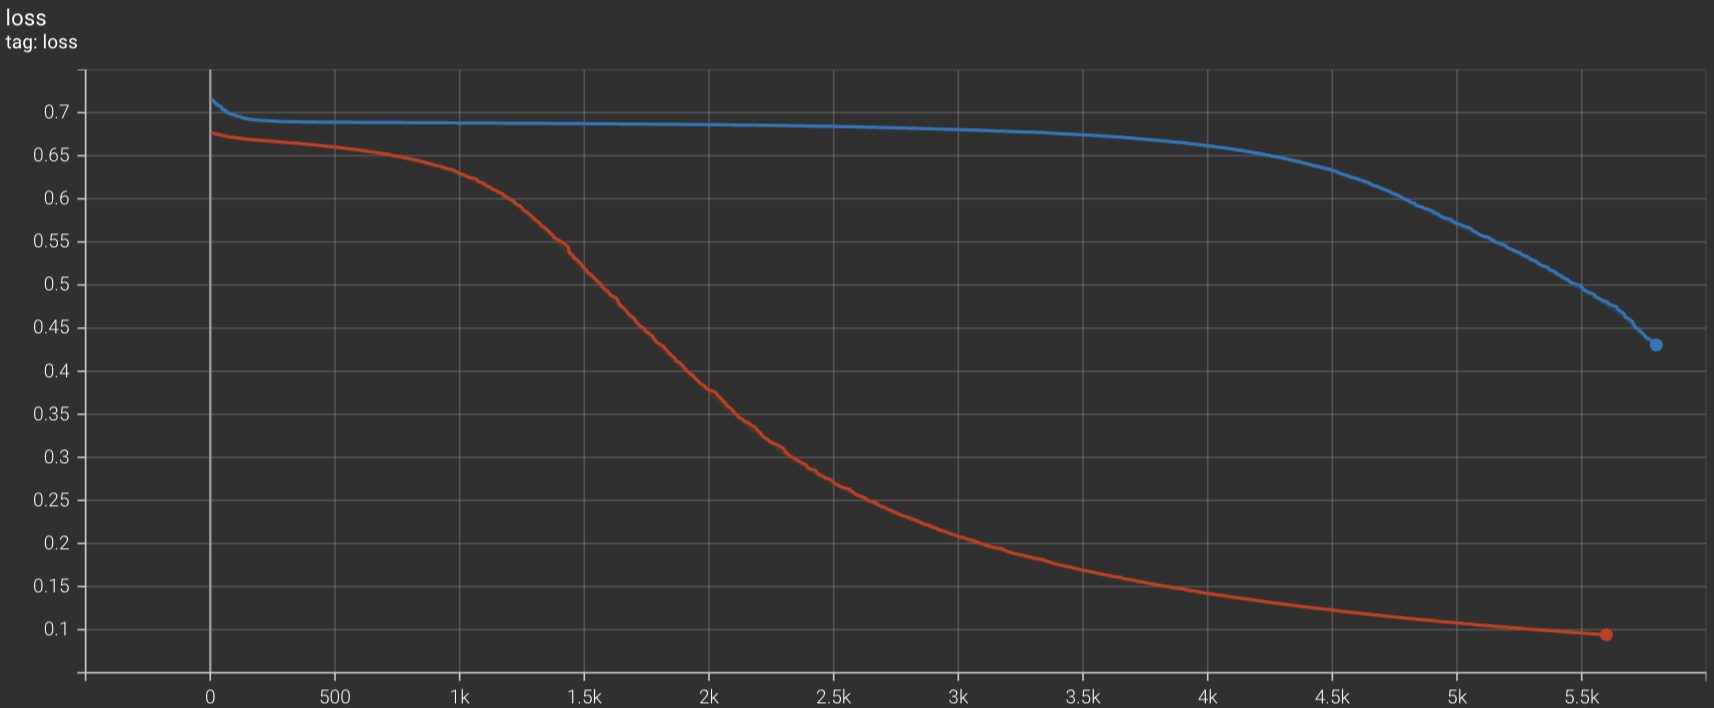
\includegraphics[scale=0.5]{img/vanilla_loss.png}
		\caption{Loss with SGD optimizer.}
		\label{optim-loss-vanilla}
	\end{figure}

\section{Different activation functions}
\indent
	Experiments of this section are done with common setup below: 
	\begin{itemize}
		\item Optimizer: \code{Adam}.
		\item Learning rate: $10^{-2}$.
		\item Dimension of hidden layers: 4.
	\end{itemize}

	From Figures \ref{result-activation-leaky-relu} and \ref{result-activation-relu}, we can see that 
	using \code{LeakyReLU} optimizer makes the model converge faster in this case.
	
	\begin{figure}[H]
		\centering
		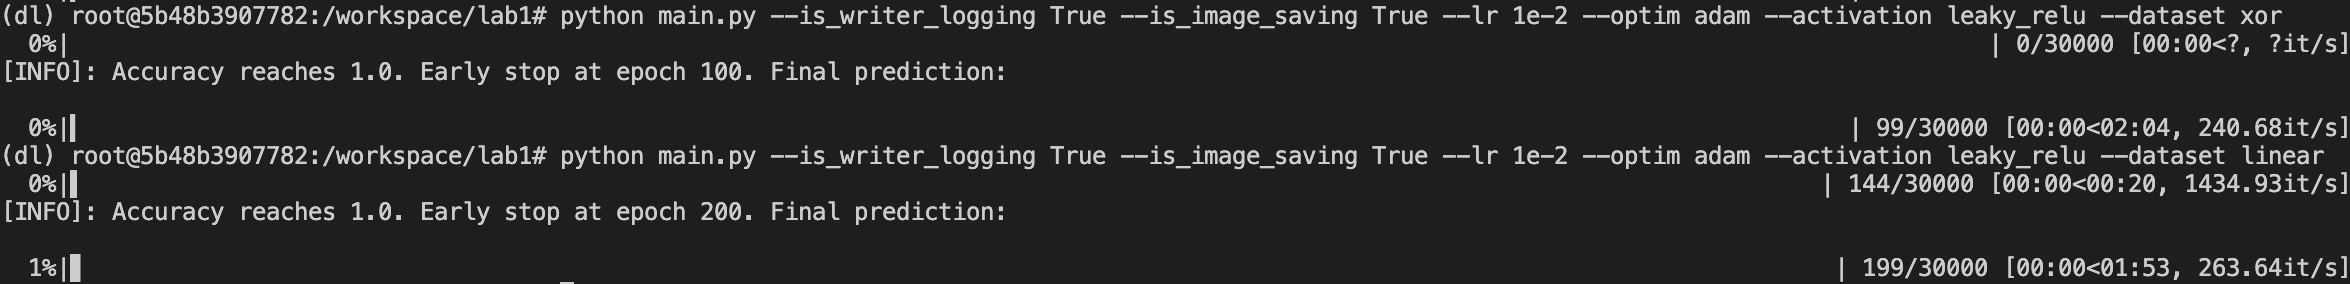
\includegraphics[scale=0.3]{img/adam_1e-2_leaky-relu.png}
		\caption{Results with LeakyReLU. In this case, the model converges in less than 100 and 200 epochs, respectively.}
		\label{result-activation-leaky-relu}
	\end{figure}
	\begin{figure}[H]
		\centering
		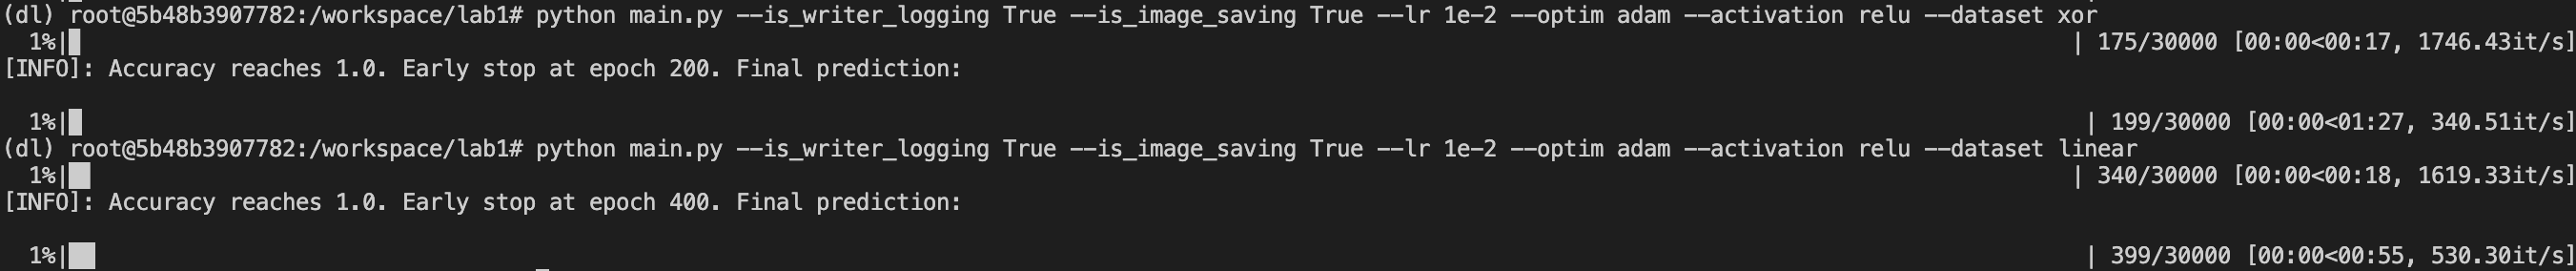
\includegraphics[scale=0.3]{img/adam_1e-2_relu.png}
		\caption{Results with ReLU. In this case, the model converges in less than 200 and 400 epochs, respectively.}
		\label{result-activation-relu}
	\end{figure}

	\begin{figure}[H]
		\centering
		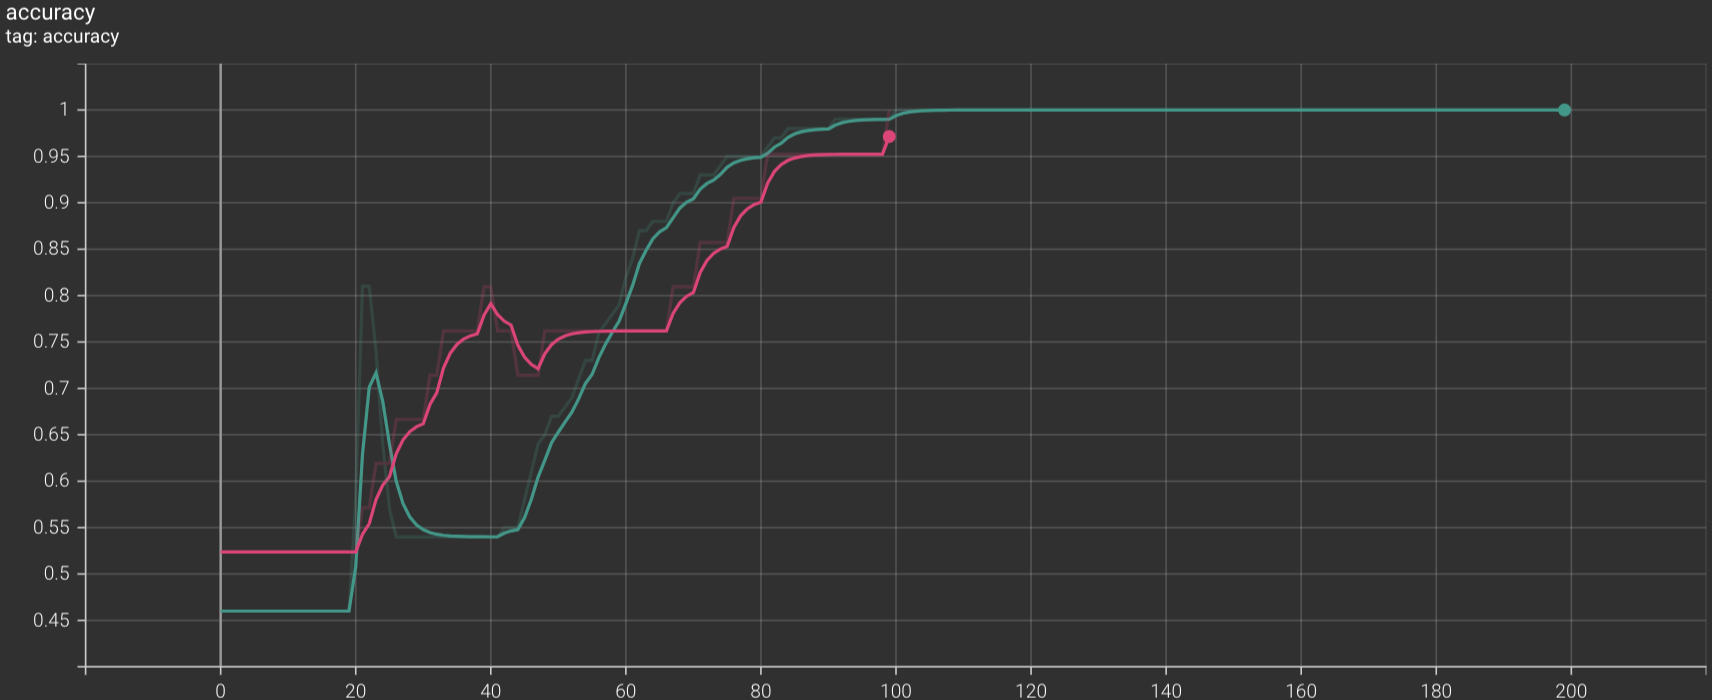
\includegraphics[scale=0.5]{img/adam_acc.png}
		\caption{Accuracy with LeakyReLU.}
		\label{activation-acc-leaky-relu}
	\end{figure}
	\begin{figure}[H]
		\centering
		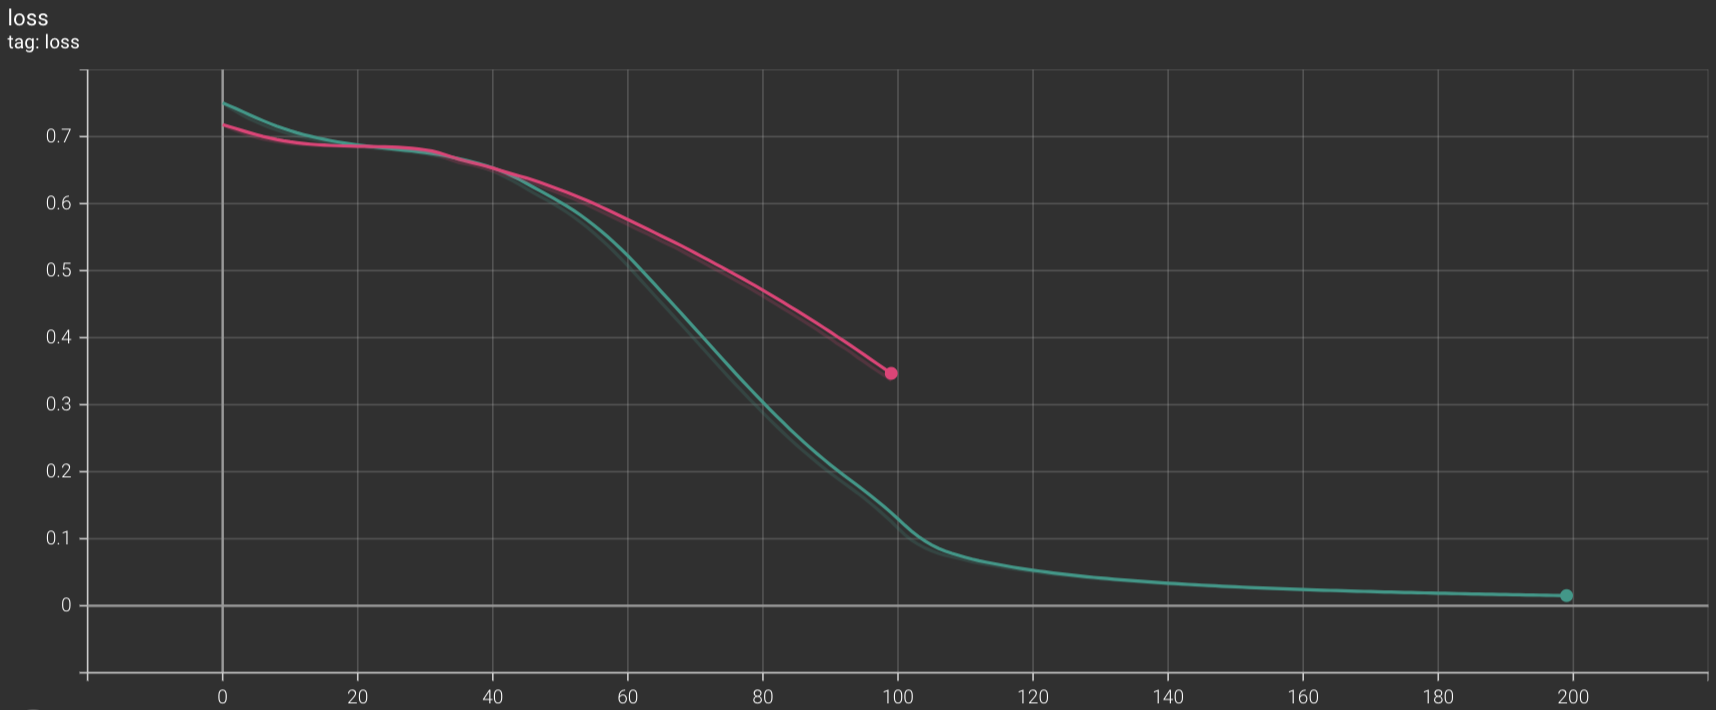
\includegraphics[scale=0.5]{img/adam_loss.png}
		\caption{Loss with LeakyReLU.}
		\label{activation-loss-leaky-relu}
	\end{figure}

	\begin{figure}[H]
		\centering
		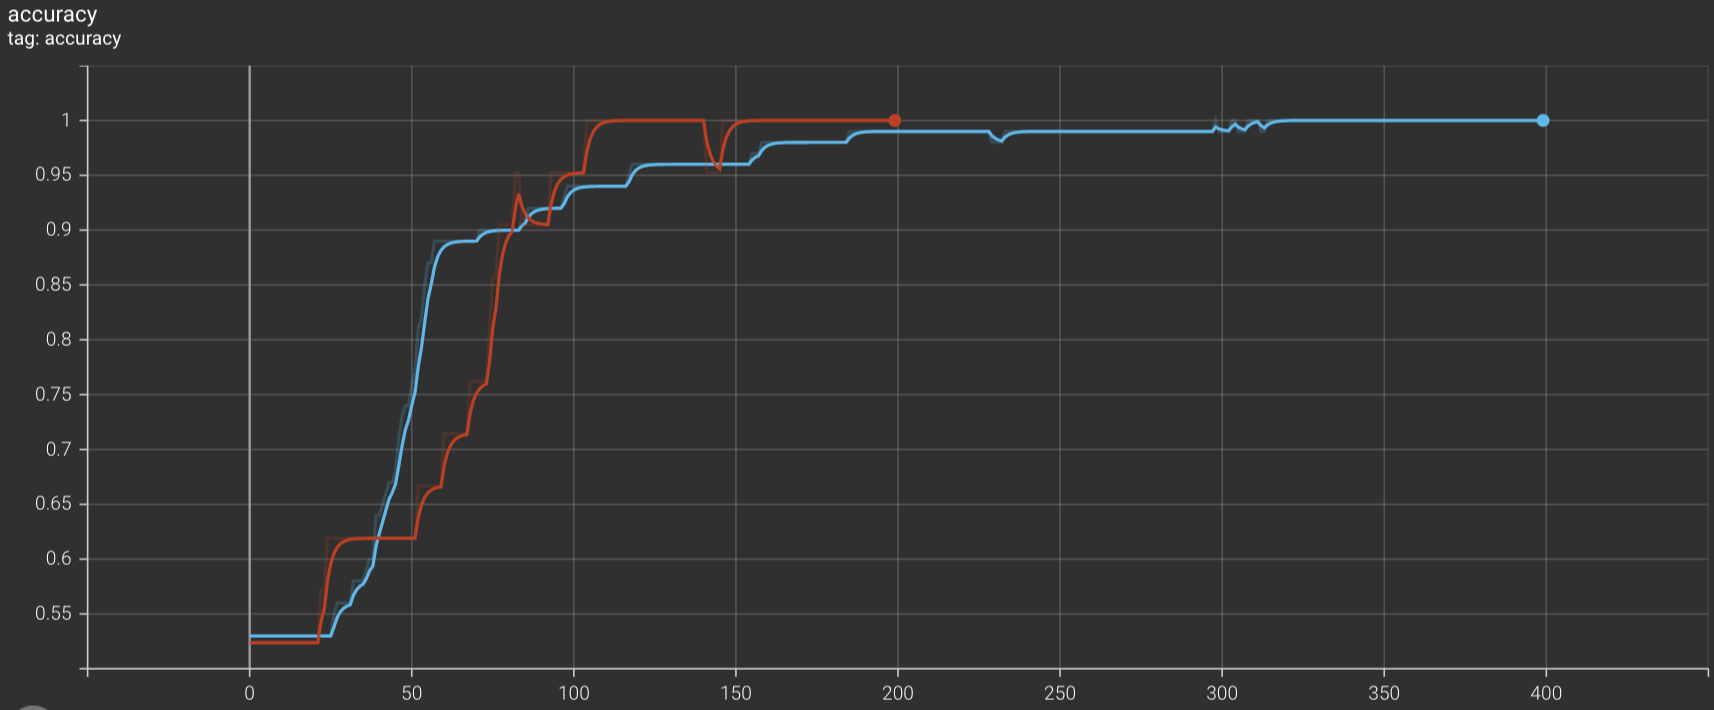
\includegraphics[scale=0.5]{img/relu_acc.png}
		\caption{Accuracy with ReLU.}
		\label{activation-acc-relu}
	\end{figure}
	\begin{figure}[H]
		\centering
		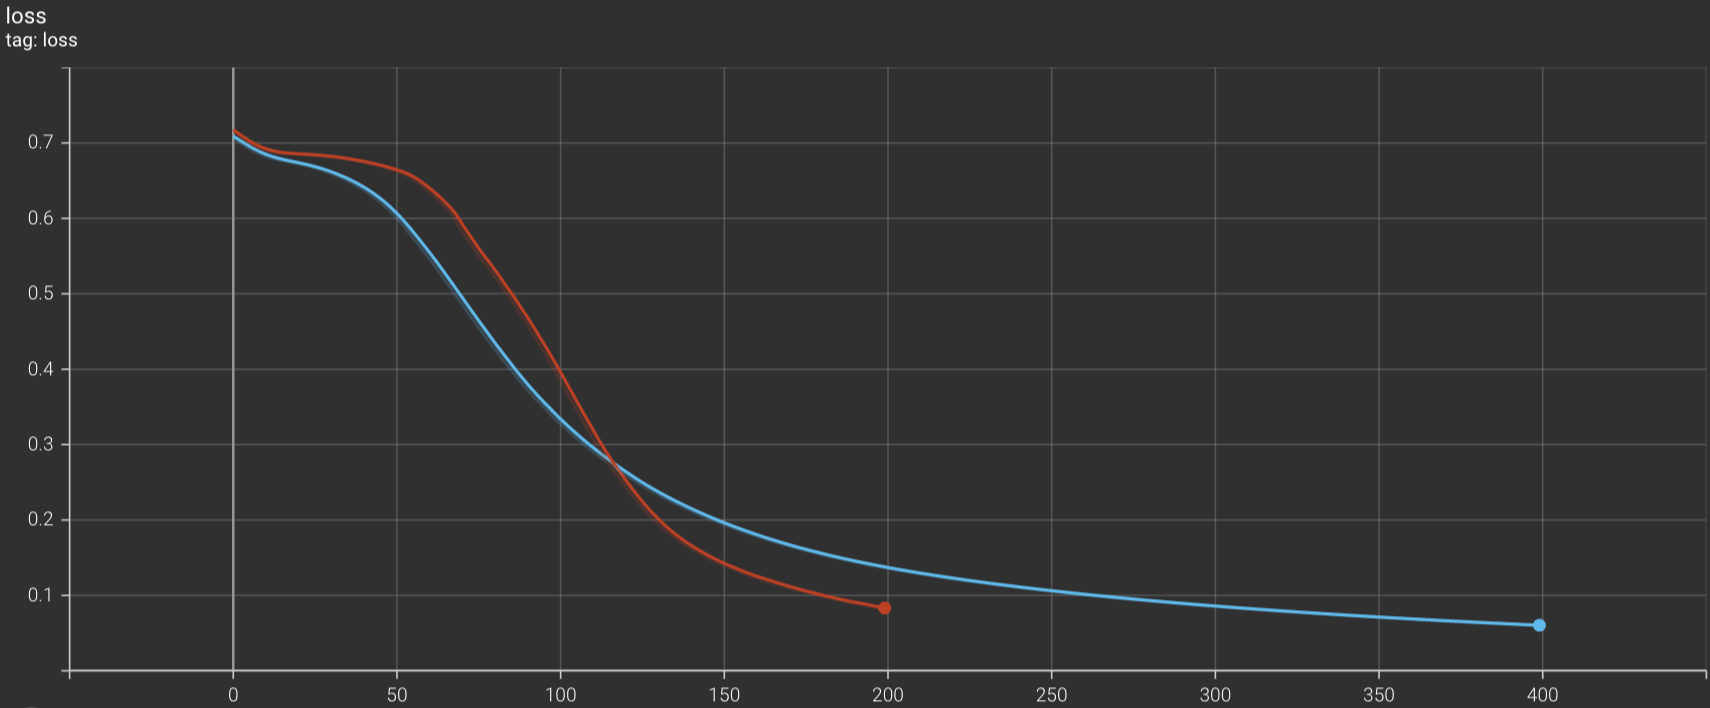
\includegraphics[scale=0.5]{img/relu_loss.png}
		\caption{Loss with ReLU.}
		\label{activation-loss-relu}
	\end{figure}

\section{Different learning rates}
\indent
	Experiments of this section are done with common setup below: 
	\begin{itemize}
		\item Optimizer: \code{Adam}.
		\item Activation function: \code{LeakyReLU}.
		\item Dimension of hidden layers: 4.
	\end{itemize}

	From Figures \ref{result-lr-1e-2} and \ref{result-lr-1e-4}, we can see that 
	using learning rate $10^{-2}$ makes the model converge faster in this case.
	
	\begin{figure}[H]
		\centering
		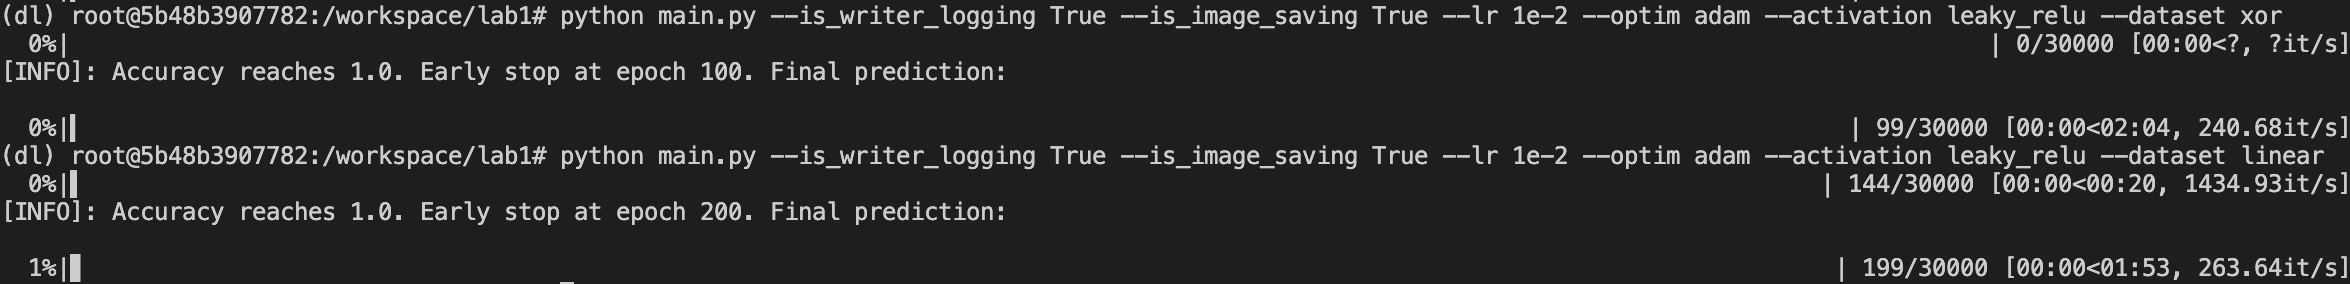
\includegraphics[scale=0.3]{img/adam_1e-2_leaky-relu.png}
		\caption{Results with learning rate $10^{-2}$. In this case, the model converges in less than 100 and 200 epochs, respectively.}
		\label{result-lr-1e-2}
	\end{figure}
	\begin{figure}[H]
		\centering
		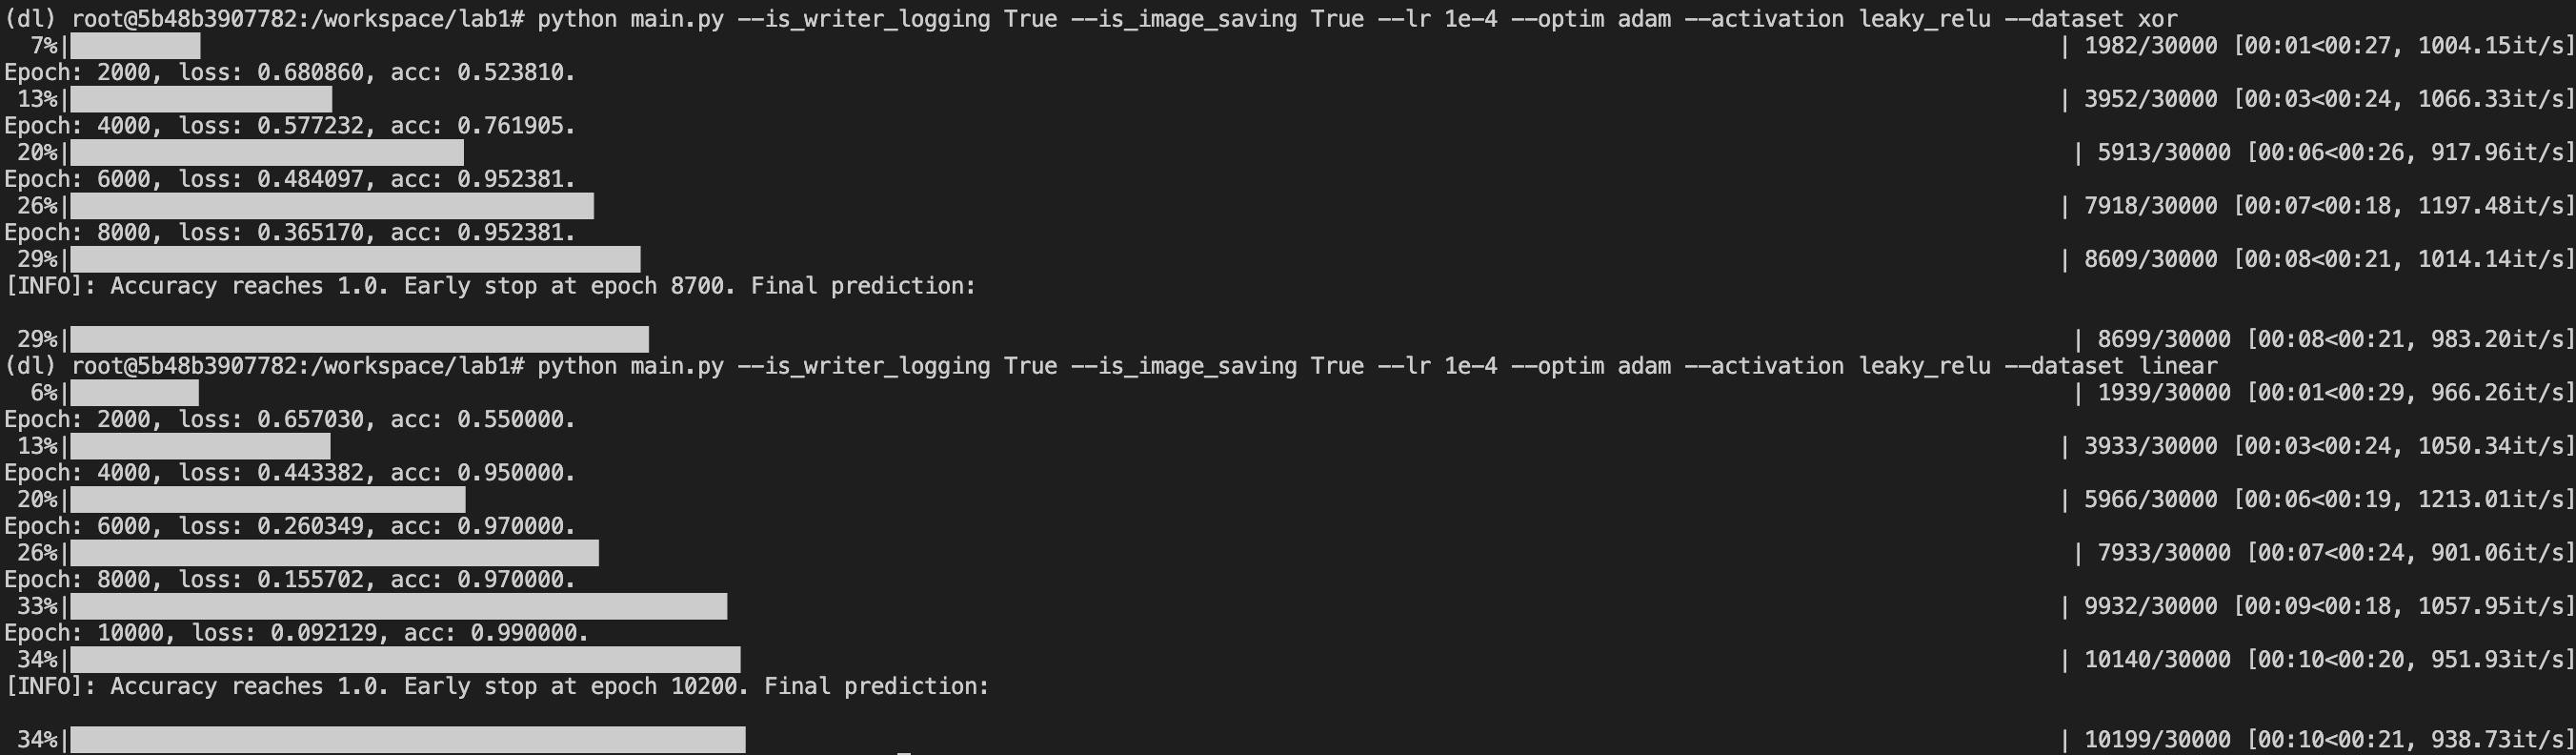
\includegraphics[scale=0.3]{img/adam_1e-4_leaky-relu.png}
		\caption{Results with learning rate $10^{-4}$. In this case, the model converges in less than 8700 and 10200 epochs, respectively.}
		\label{result-lr-1e-4}
	\end{figure}

	\begin{figure}[H]
		\centering
		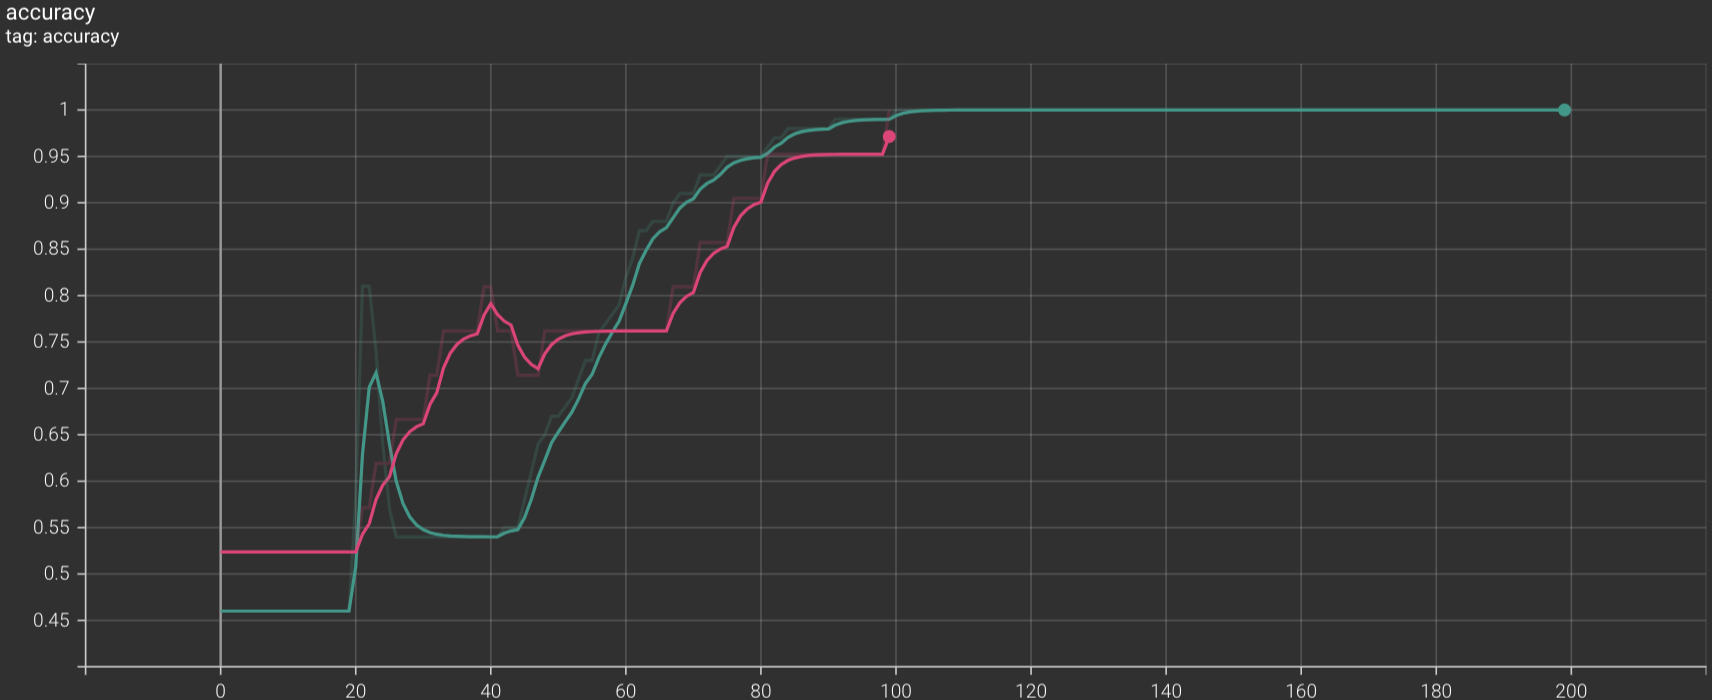
\includegraphics[scale=0.5]{img/adam_acc.png}
		\caption{Accuracy with learning rate $10^{-2}$.}
		\label{lr-acc-1e-2}
	\end{figure}
	\begin{figure}[H]
		\centering
		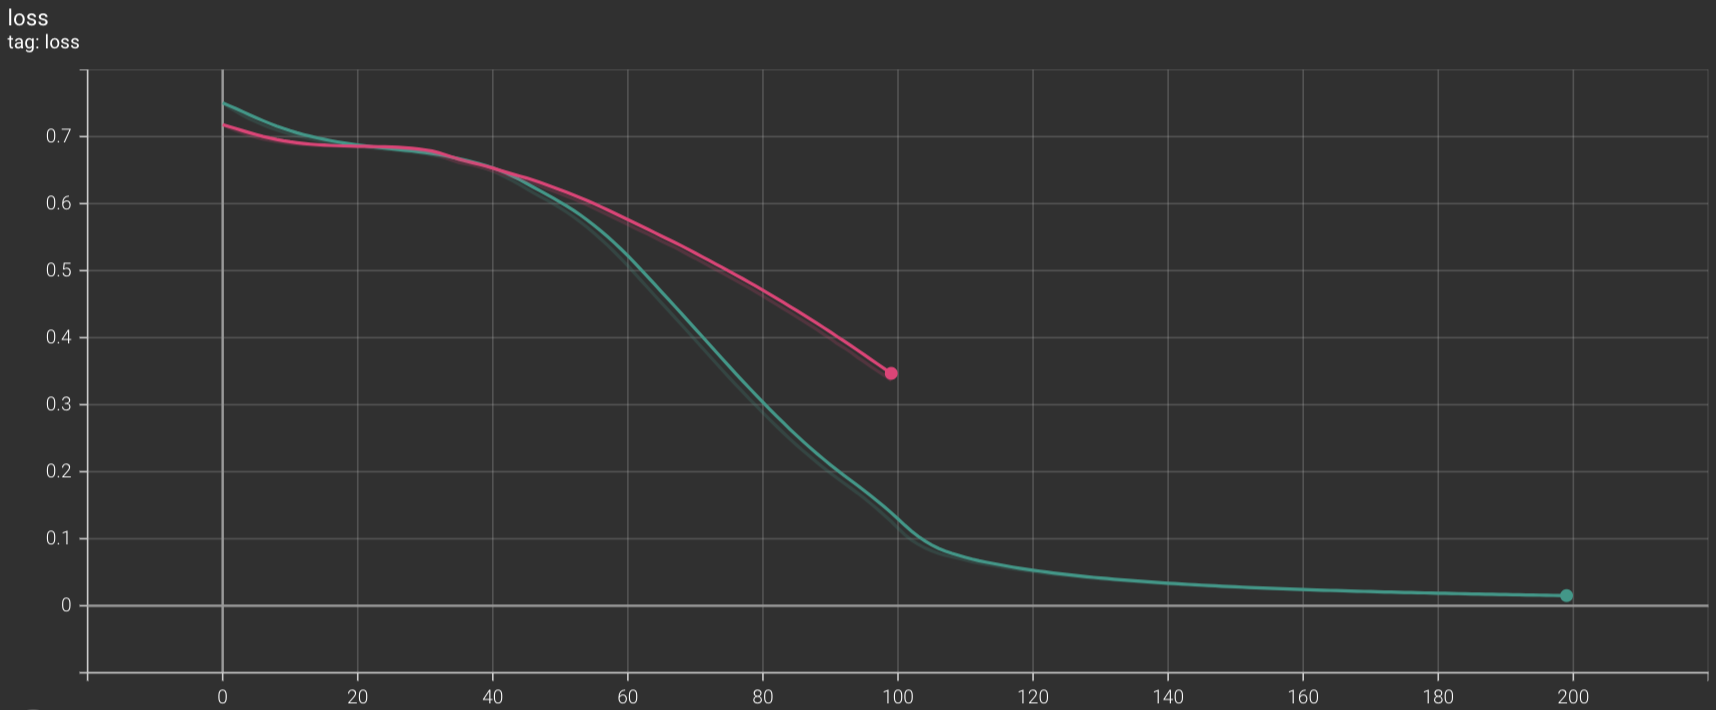
\includegraphics[scale=0.5]{img/adam_loss.png}
		\caption{Loss with learning rate $10^{-2}$.}
		\label{lr-loss-1e-2}
	\end{figure}

	\begin{figure}[H]
		\centering
		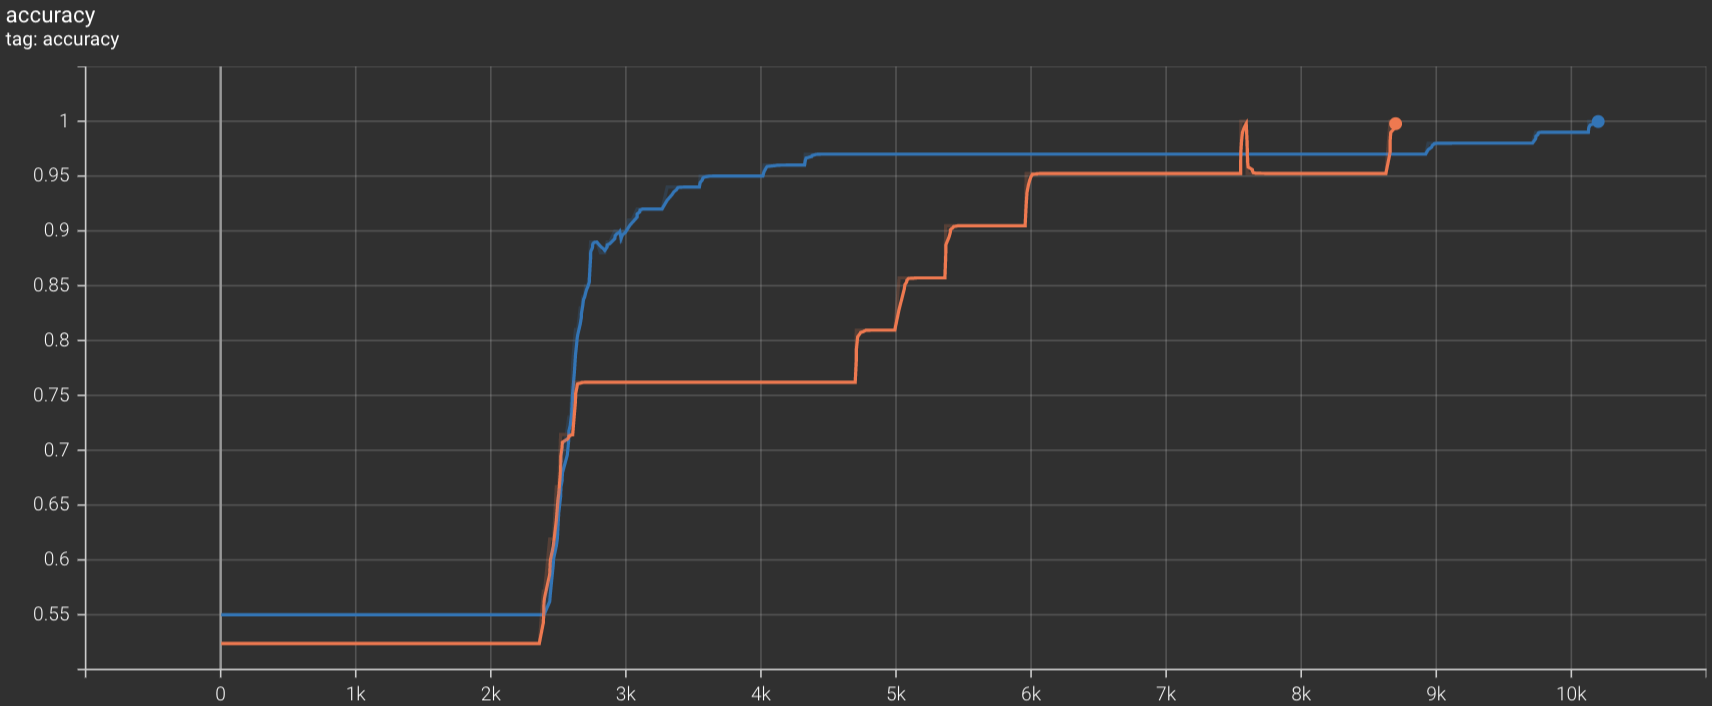
\includegraphics[scale=0.5]{img/1e-4_acc.png}
		\caption{Accuracy with learning rate $10^{-4}$.}
		\label{lr-acc-1e-4}
	\end{figure}
	\begin{figure}[H]
		\centering
		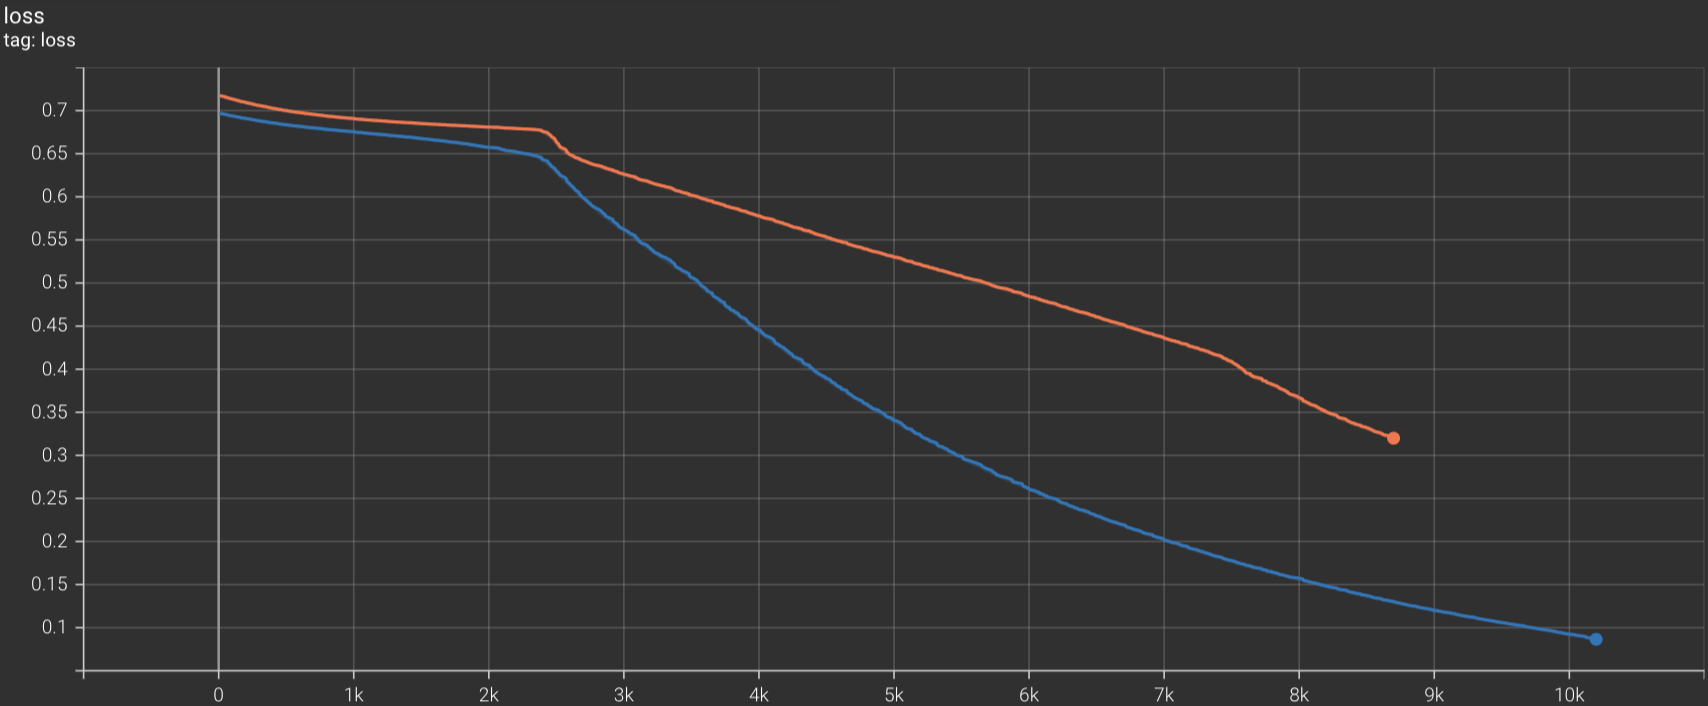
\includegraphics[scale=0.5]{img/1e-4_loss.png}
		\caption{Loss with learning rate $10^{-4}$.}
		\label{lr-loss-1e-4}
	\end{figure}

\section{Different dimension of hidden layers}
\indent
	Experiments of this section are done with common setup below: 
	\begin{itemize}
		\item Optimizer: \code{Adam}.
		\item Activation function: \code{LeakyReLU}.
		\item Learning rate: $10^{-2}$.
	\end{itemize}

	From Figures \ref{result-dim-4} and \ref{result-dim-16}, we can see that 
	using 16-dimension hidden layers makes the model converge faster in this case.
	
	\begin{figure}[H]
		\centering
		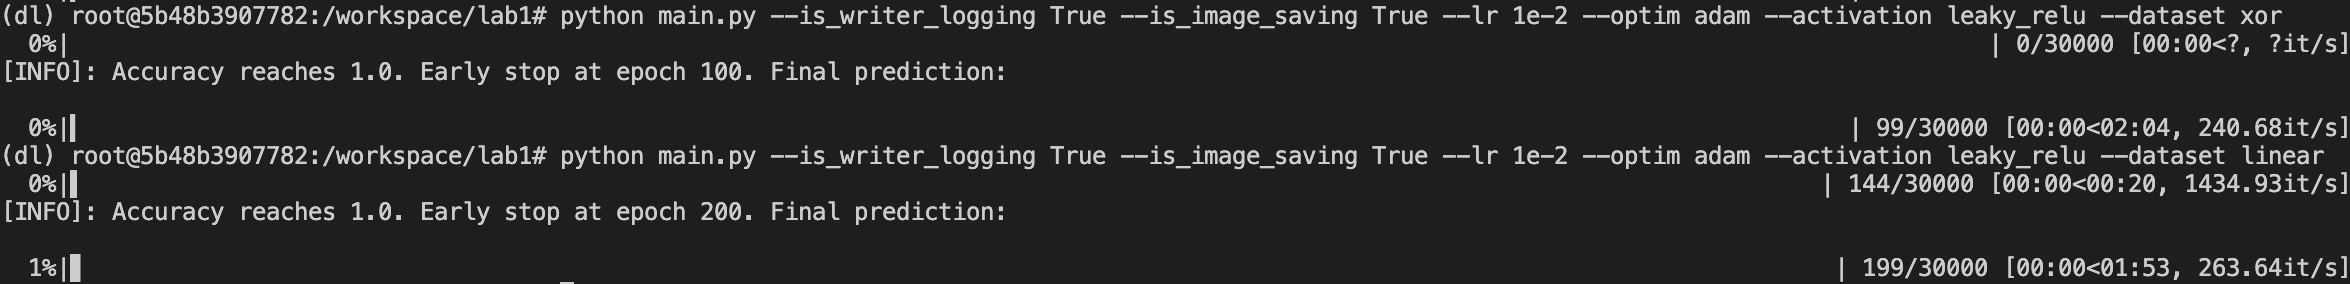
\includegraphics[scale=0.3]{img/adam_1e-2_leaky-relu.png}
		\caption{Results with 4-dimension hidden layers. In this case, the model converges in less than 100 and 200 epochs, respectively.}
		\label{result-dim-4}
	\end{figure}
	\begin{figure}[H]
		\centering
		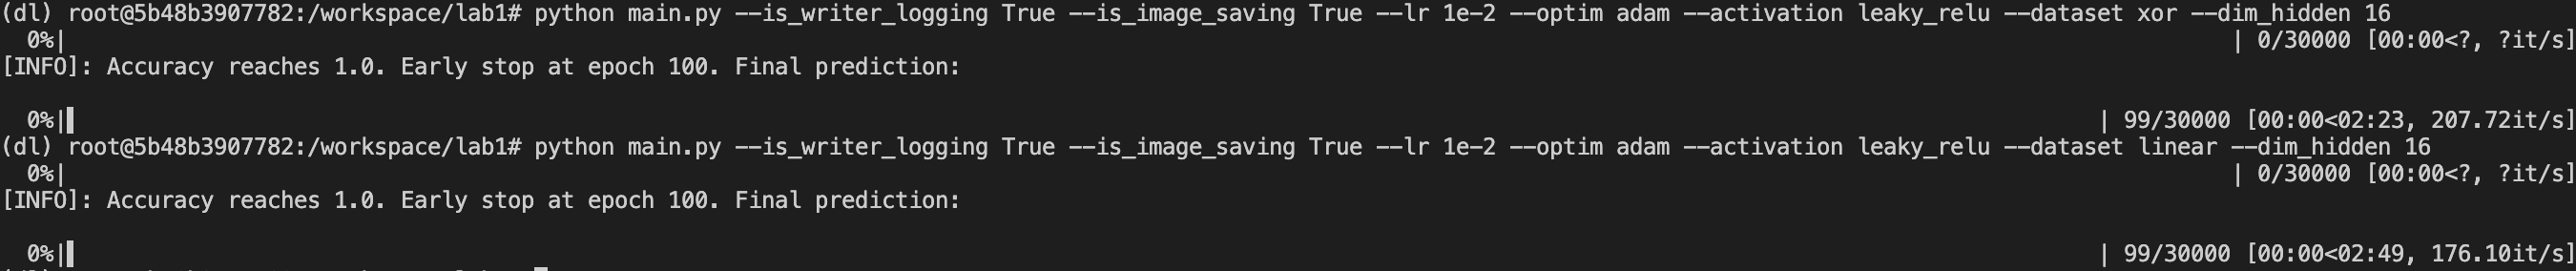
\includegraphics[scale=0.3]{img/adam_1e-2_leaky-relu_16.png}
		\caption{Results with 16-dimension hidden layers. In this case, the model converges in less than 100 and 100 epochs, respectively.}
		\label{result-dim-16}
	\end{figure}

	\begin{figure}[H]
		\centering
		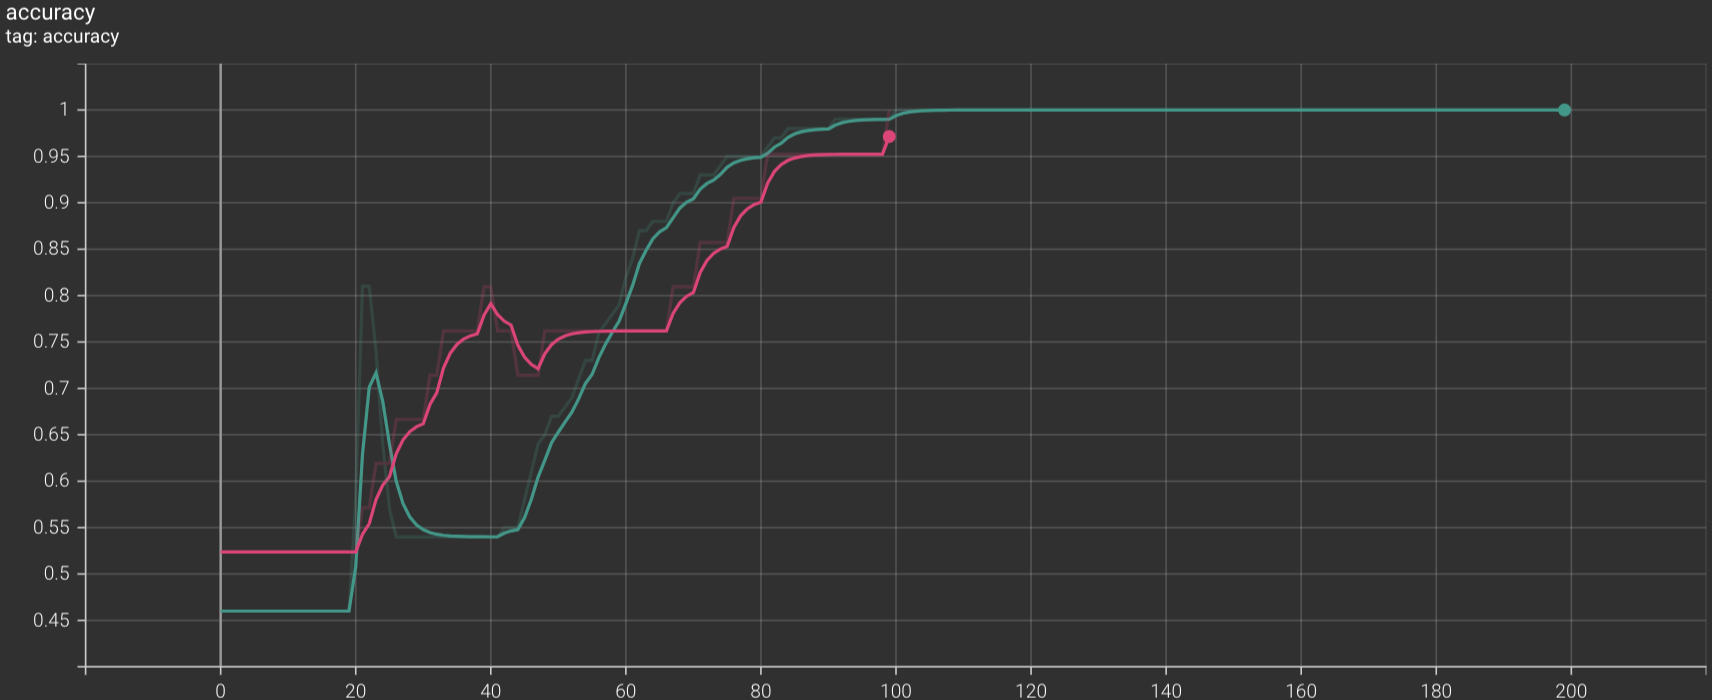
\includegraphics[scale=0.5]{img/adam_acc.png}
		\caption{Accuracy with 4-dimension hidden layers.}
		\label{dim-acc-4}
	\end{figure}
	\begin{figure}[H]
		\centering
		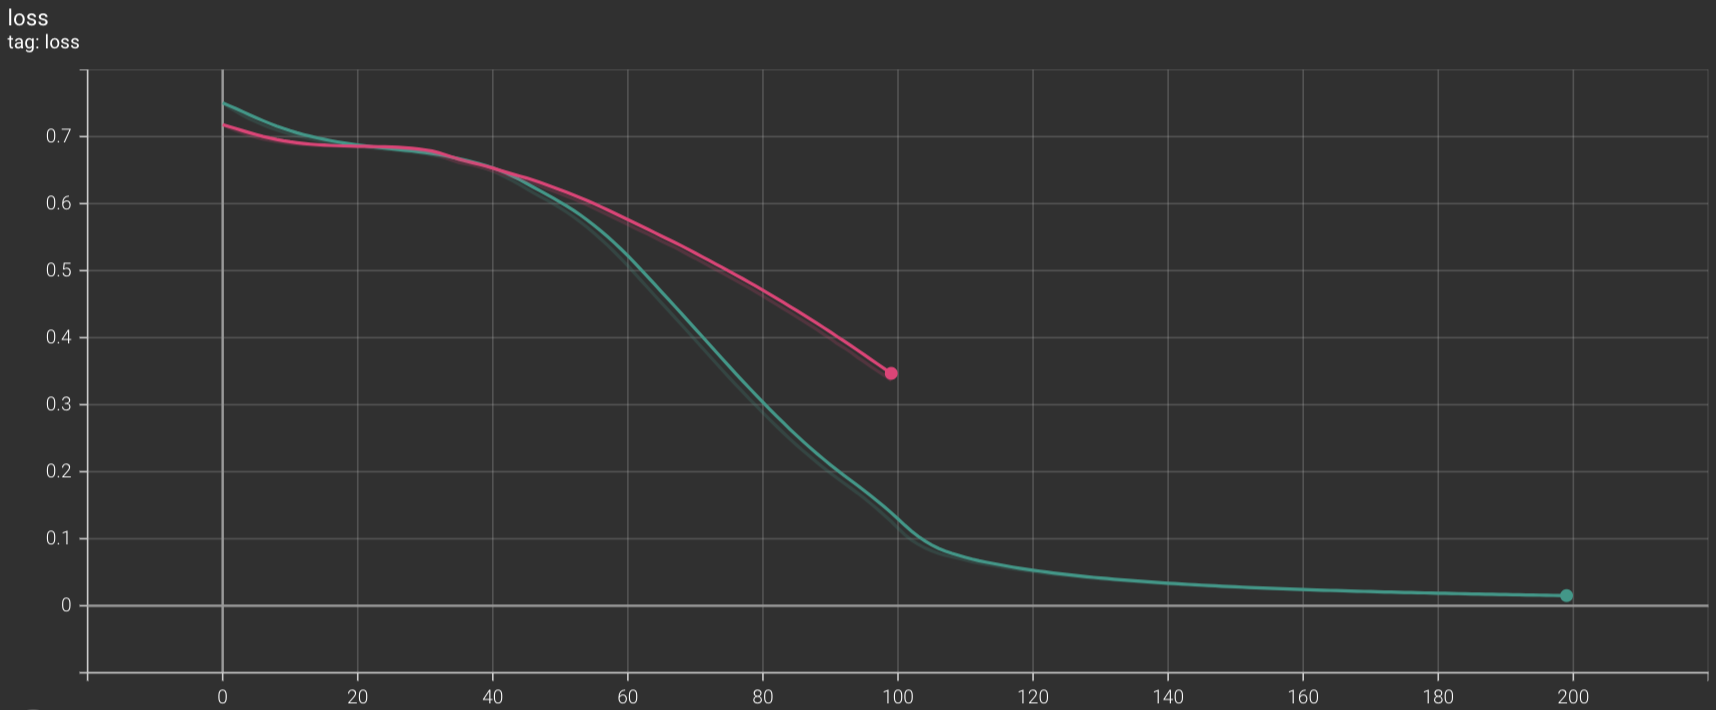
\includegraphics[scale=0.5]{img/adam_loss.png}
		\caption{Loss with 4-dimension hidden layers.}
		\label{dim-loss-4}
	\end{figure}

	\begin{figure}[H]
		\centering
		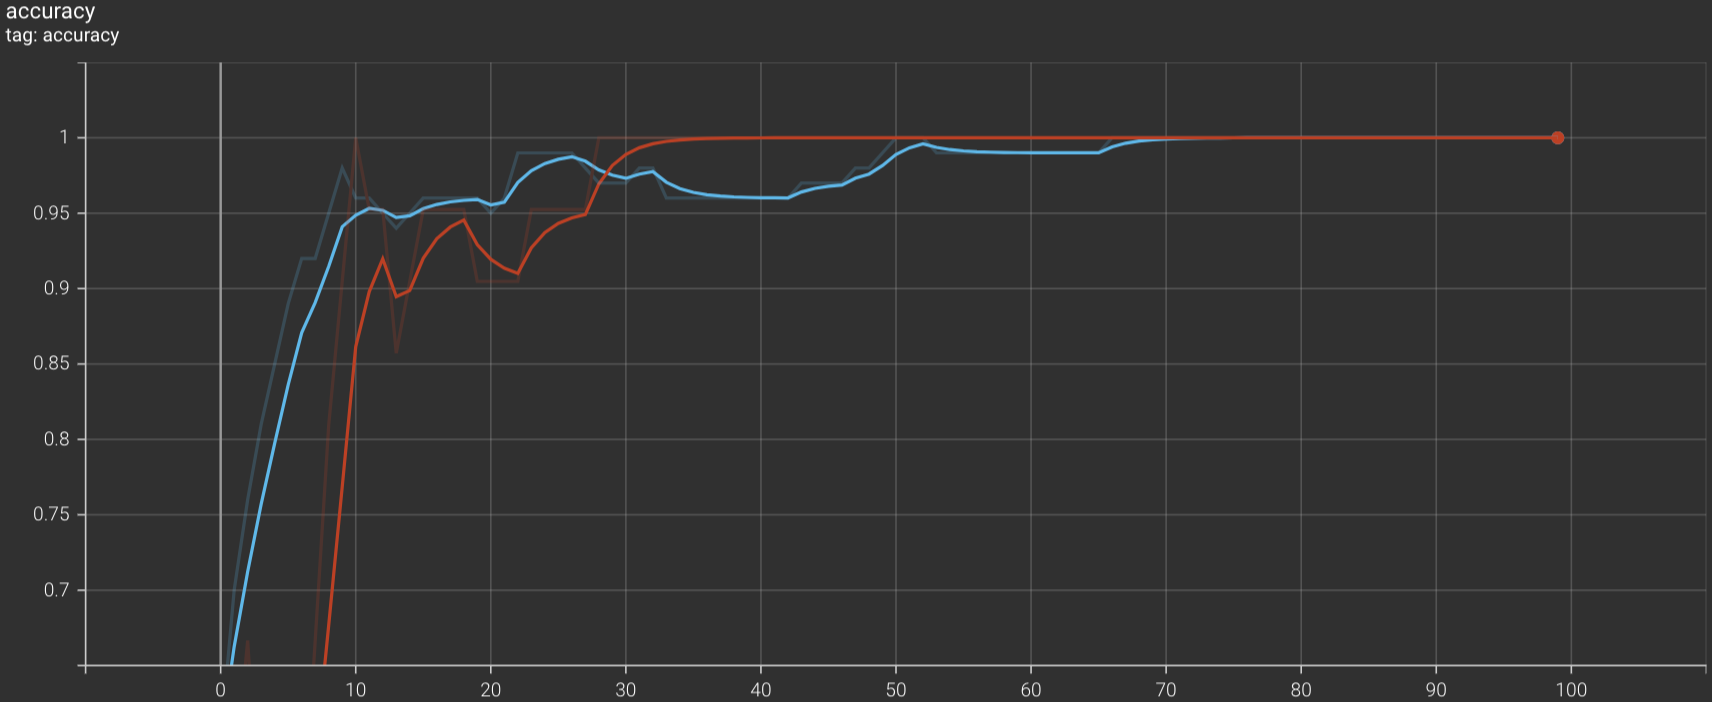
\includegraphics[scale=0.5]{img/acc_16.png}
		\caption{Accuracy with 16-dimension hidden layers.}
		\label{dim-acc-16}
	\end{figure}
	\begin{figure}[H]
		\centering
		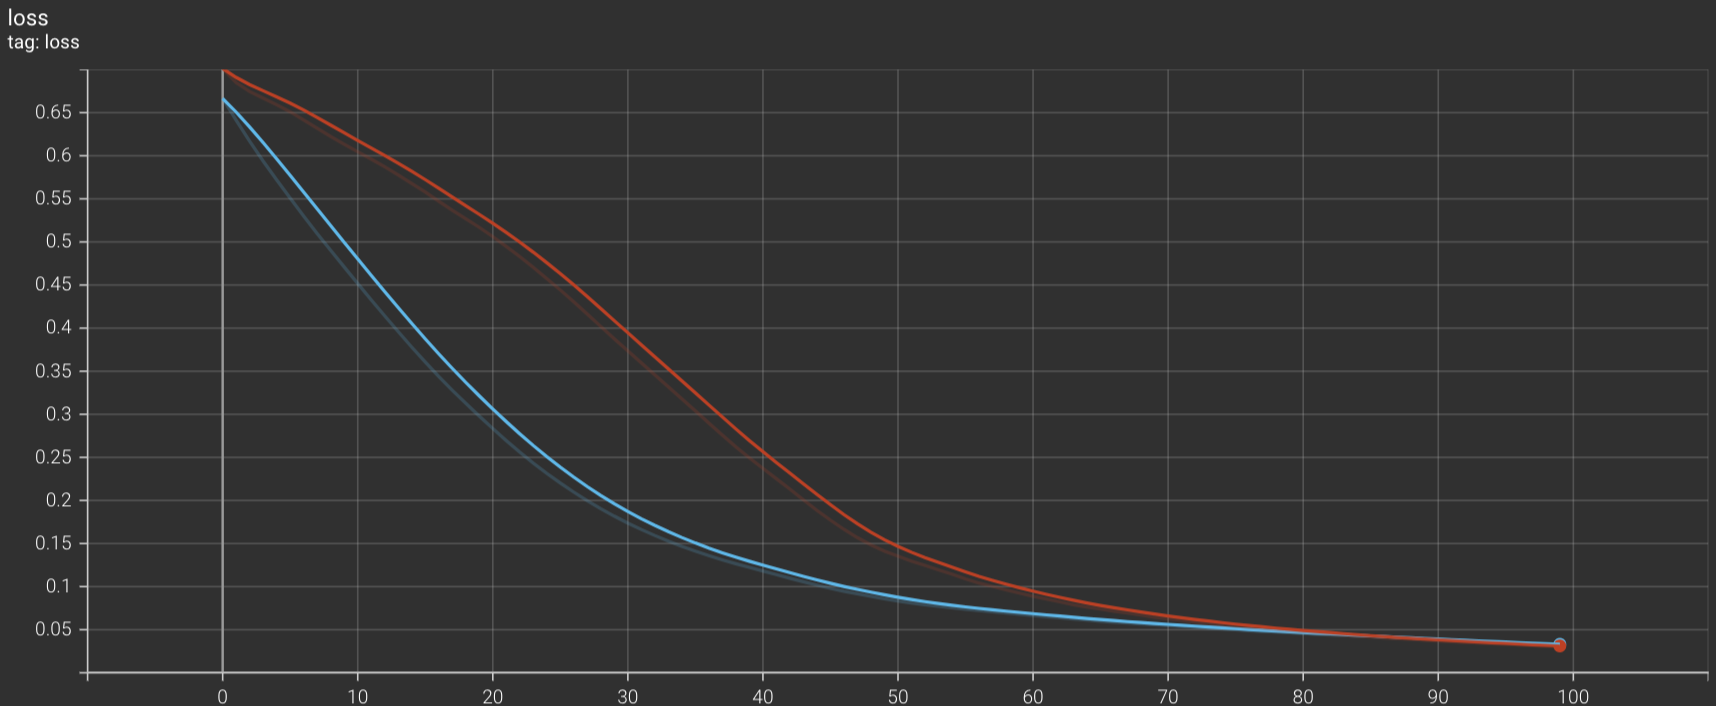
\includegraphics[scale=0.5]{img/loss_16.png}
		\caption{Loss with 16-dimension hidden layers.}
		\label{dim-loss-16}
	\end{figure}